\section{Wstęp}

\indent Niniejsze opracowanie dotyczy projektu oprogramowania systemu, którego zadaniem jest automatyczne wyznaczanie nastaw dla regulatora silników DC oraz ich optymalizacja względem określonego kryterium. 
\newline Przedstawiony w specyfikacji funkcjonalnej system umożliwiać będzie realizację następujących zadań :
\begin{itemize}
\item wprowadzanie przez użytkownika wymaganych parametrów silnika prądu stałego,
\item automatyczną identyfikację parametrów silnika prądu stałego,
\item wyznaczanie nastaw regulatora na podstawie zadanej trajektorii odpowiedzi silnika,
\item optymalizacja nastaw za pomocą algorytmu genetycznego i danych z rzeczywistego obiektu,
\item wizualizacja wartości wielkości pomiarowych podczas pracy silnika.
\end{itemize}
Poniżej przedstawiono specyfikacje funkcjonalną systemu w której zdefiniowano klienta oraz użytkowników końcowych systemu, przedstawiono wymagania funkcjonalne oraz scenariusze użycia systemu.
\section{Specyfikacja funkcjonalna}
\subsection{Identyfikacja klienta oraz użytkowników końcowych}
\indent Potencjalnym klientem dla omawianego systemu mogą być wszelkie firmy i zakłady produkcyjne, które posiadają w swych liniach technologicznych napędy wykorzystujące silniki prądu stałego. Z racji podobnych, docelowych warunków pracy i realizowanych zadań systemu, firma ta może zajmować się produkcją układów elektronicznych lub mechanicznych, których proces technologiczny wymaga realizacji określonego ruchu z zadanymi parametrami.\newline
\indent Docelowym użytkownikiem systemu będzie więc osoba na stanowisku technika utrzymania ruchu lub inżyniera automatyka, której zadaniem jest przygotowanie odpowiedniego układu sterowania silnikiem DC, umożliwiającego realizację zadanych przemieszczeń elementów maszyn. \newline
\indent Zaletą systemu z punktu widzenia potencjalnego klienta - firmy produkcyjnej, jest znaczne ułatwienie i uproszczenie skomplikowanego procesu strojenia regulatorów napędów, a co za tym idzie otrzymanie zadowalających wyników i efektów sterowania w procesie produkcyjnym, bez potrzeby zatrudnienia wysoko i ściśle wykwalifikowanej kadry inżynierów.\newline
\indent Podsumowując, dla omawianego systemu zdefiniować można następujące warunki docelowe:
\begin{itemize}
\item \textbf{Potencjalny klient} - firma produkcyjna Drutex,
\item \textbf{Docelowe środowisko pracy} - hala produkcyjna, otoczenie zautomatyzowanej linii technologicznej,
\item \textbf{Użytkownik końcowy} - dorosła osoba na stanowisku technika lub inżyniera utrzymania ruchu.
\end{itemize}
\newpage
\subsection{Wymagania funkcjonalne i pozafunkcjonalne systemu}

\indent Na podstawie ogólnej koncepcji założeń  pracy systemu, zdefiniowano jego komponenty składowe, wymagania fukcjonalne i pozafunkcjonalne które opisują cechy oprogramowania i zadania które powinno ono realizować. \newline
\indent W strukturze omawianego systemu wyszczególnić można następujące komponenty składowe:
\begin{itemize}
\item \textbf{użytkownik} - osoba na stanowisku technika utrzymania ruchu,
\item \textbf{urządzenie HMI} - komputer PC, laptop lub tablet umożliwiający uruchomienie aplikacji i komunikację z użytkownikiem,
\item \textbf{aplikacja} - główny program realizujący zadanie optymalizacji nastaw, uruchomiony na urządzeniu HMI,
\item \textbf{sterownik PLC} - podrzędne urządzenie skomunikowane z HMI, wykonujące zadania sterująco-pomiarowe na silniku DC,
\item \textbf{silnik DC} - docelowy obiekt rzeczywisty.
\end{itemize}

\vspace{0.4cm}
\indent Dla omawianego systemu określono wymagania funkcjonalne, definiujące zadania realizowane przez poszczególne komponenty składowe oraz zintegrowaną całość :


\begin{enumerate}
\item Główną funkcjonalnością systemu jest wyznaczenie optymalnych nastaw regulatora PID w systemie sterowania prędkością silnika prądu stałego.
\item Parametry modelu silnika mogą być wprowadzone przez operatora przy użyciu interfejsu.
\item W przypadku nieposiadania przez operatora parametrów silnika, system powinien umożliwiać odczyt niezbędnych parametrów (np. stałej czasowej mechanicznej) z rzeczywistego modelu silnika, przy użyciu sterownika PLC.
\item Aplikacja powinna posiadać możliwość generowania wykresów przedstawiających przebieg wielkości sygnałów sterujących i pomiarowych.
\item System powinien zapewniać komunikację ze sterownikiem PLC odpowiedzialnym za sterowanie silnikiem i pomiar jego parametrów.
\item Aplikacja oprócz optymalizacji sterowania na modelu symulacyjnym, powinna umożliwiać weryfikacje otrzymanych wyników na obiekcie rzeczywistym i uwzględnienie ewentualnych odchyłek.
\end{enumerate}
\vspace{0.4cm}
\indent Wymagania pozafunkcjonalne zdefiniowane dla omawianego systemu są następujące:
\begin{enumerate}
\item Aplikacja powinna posiadać czytelny dla użytkownika interfejs graficzny, umożliwiający korzystanie w warunkach przemysłowych.
\item Na wykresach przebiegów sygnałów procesowych generowanych przez aplikację, każdy z sygnałów powinien posiadać unikalny kolor.
\item Optymalne nastawy regulatora PID wyznaczane będą z wykorzystaniem algorytmu genetycznego.
\item Projektowana aplikacja powinna być przenośna pomiędzy urządzeniami takimi jak PC, laptop, tablet, posiadającymi system operacyjny Windows.
\end{enumerate}

\begin{figure}[ht!]
\centering
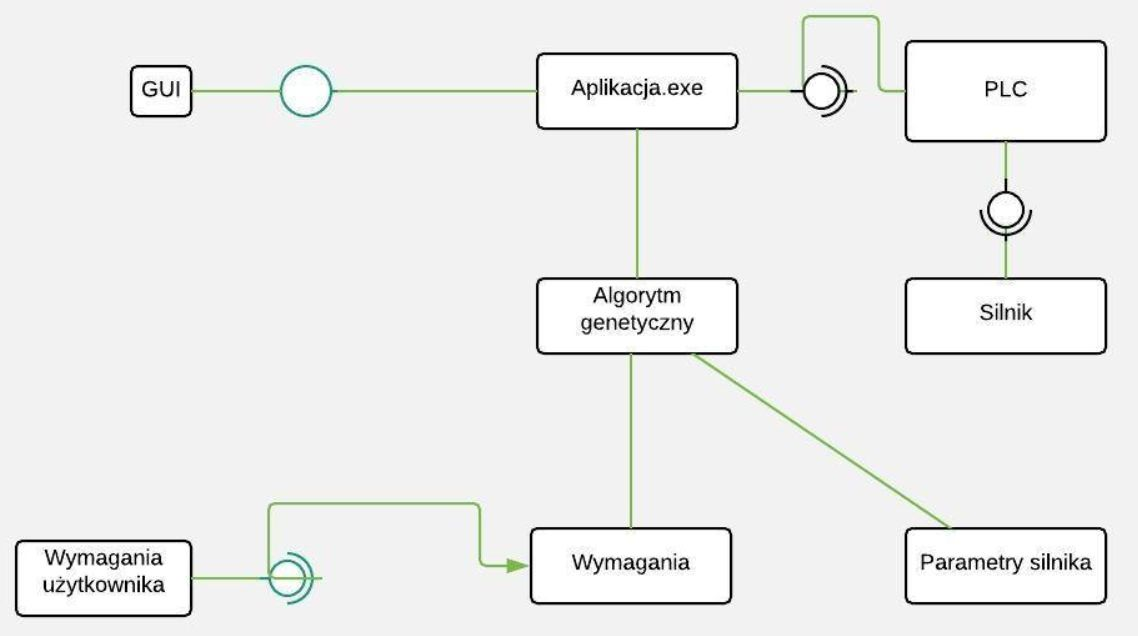
\includegraphics[scale=0.5]{komponent}
\caption{Struktura systemu i wyszczególnienie jego komponentów składowych}
\label{komponent}
\end{figure} 
\newpage
\begin{figure}[h!]
\centering
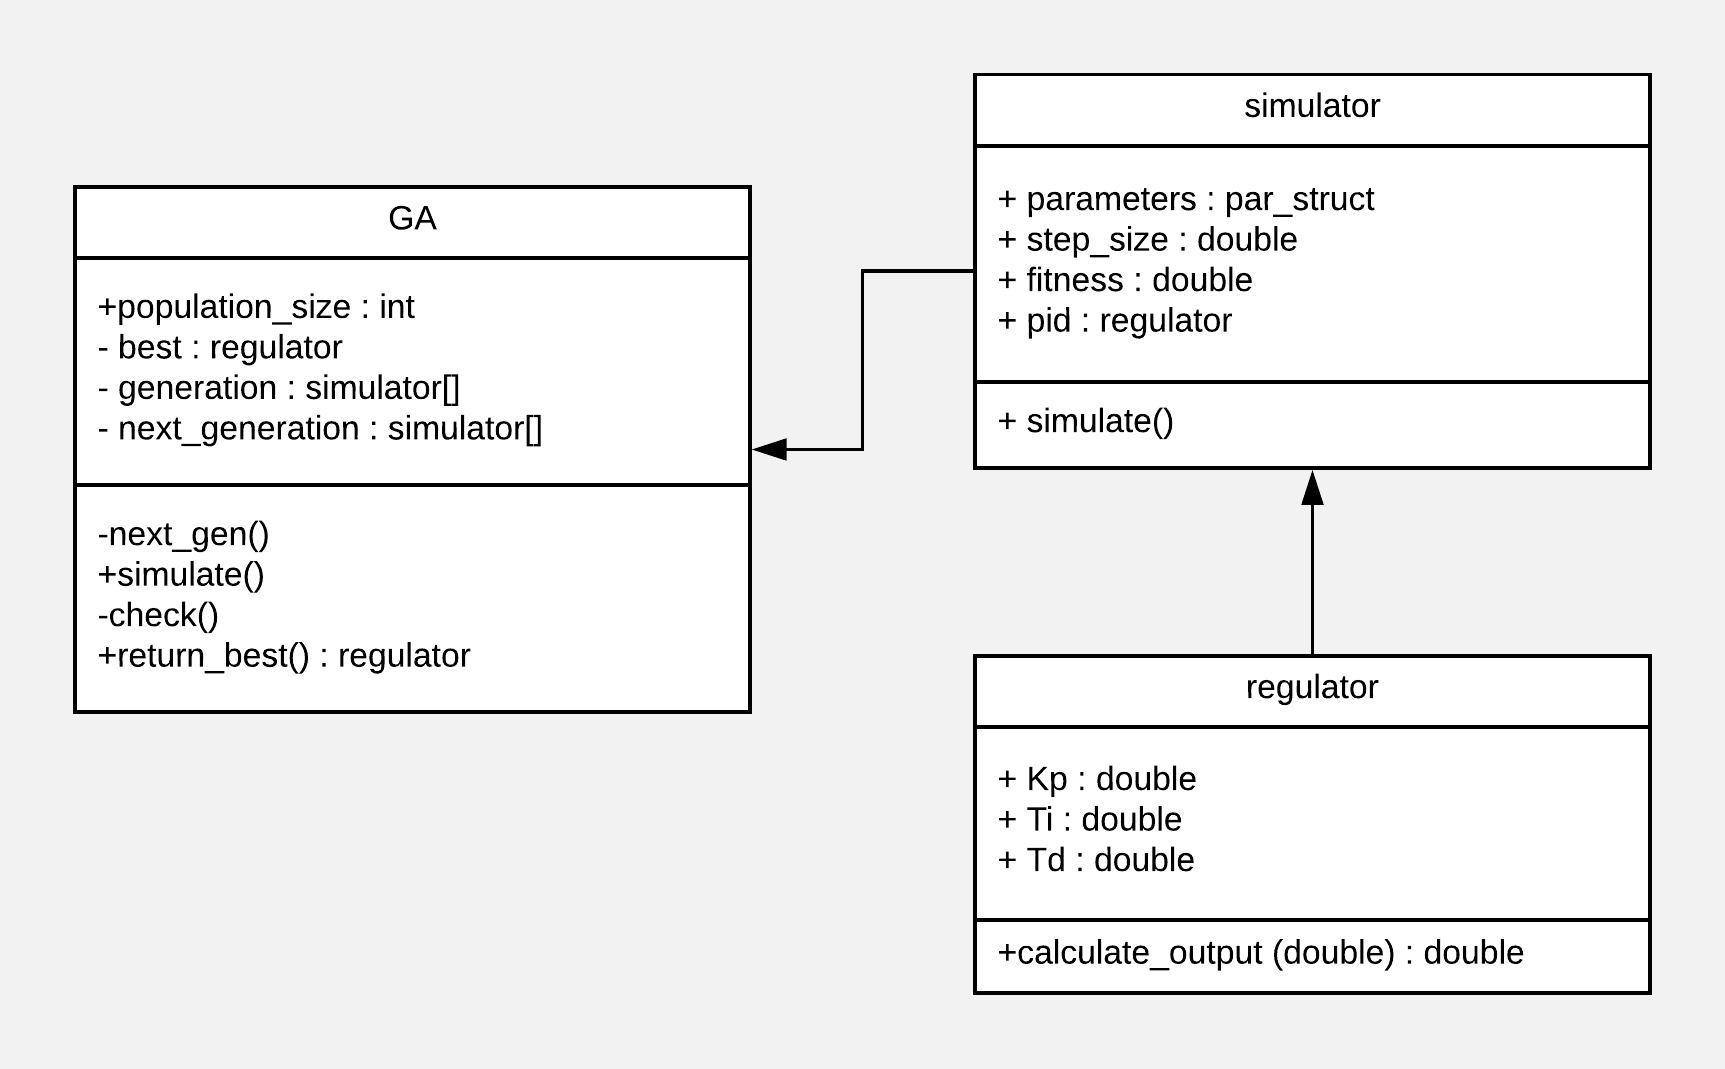
\includegraphics[scale=0.25]{klasa}
\caption{Diagram przedstawiający strukturę klas w oprogramowaniu systemu}
\label{klasa}
\end{figure}
Na rysunkach \ref{komponent} oraz \ref{klasa} przedstawiono wyszczególnione komponenty całego systemu oraz klasy składowe jego oprogramowania.\
\subsection{Scenariusze użycia systemu}
\indent Przykładowy, zakładany scenariusz użycia systemu ukazujący interakcję pomiędzy jego poszczególnymi komponentami podczas realizacji określonych zadań, przedstawiony został na rysunku \ref{aktywnosc}, znajdującym się na następnej stronie.\newpage
\begin{figure}[ht!]
\centering
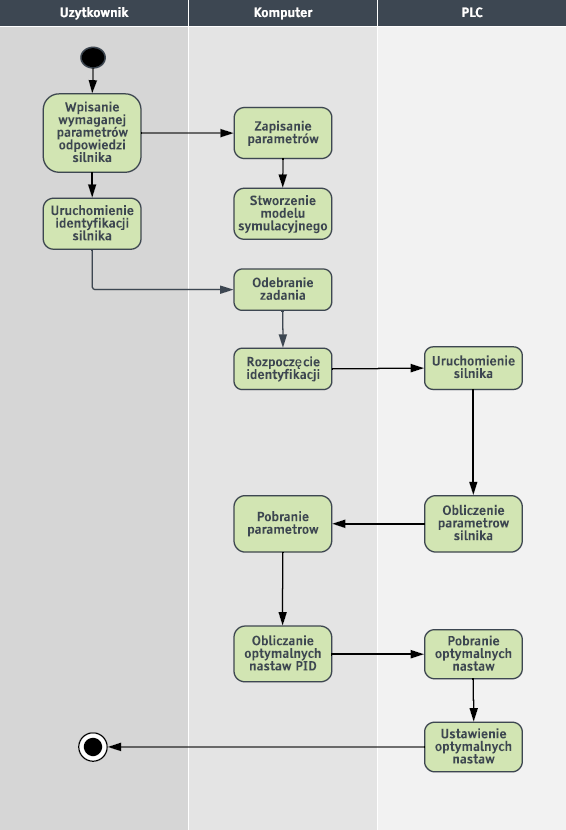
\includegraphics[scale=1]{aktywnosc}
\caption{Diagram aktywności dla omawianego systemu}
\label{aktywnosc}
\end{figure}

\newpage